\question In the figure, there is an electric field in the conducting wire due to a battery which is not shown. The wire has a mobile electron density of $n$, an electron mobility of $u$, a length $d$ and a cross-sectional area $A$. The electric field $\vec{E}=E\hat{x}$, and the charge carriers are electrons.

\begin{figure}[ht!]
	\centering
	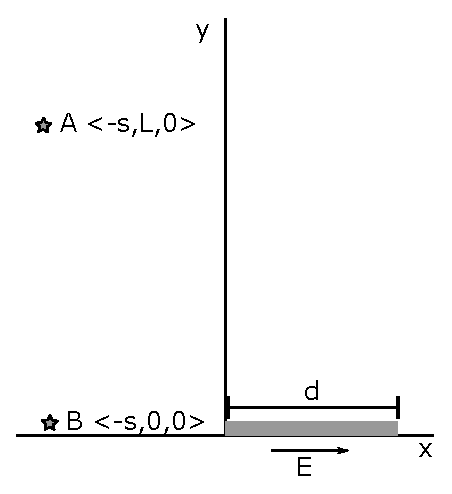
\includegraphics[width=8cm]{temp}
\end{figure}

\begin{parts}
	\part What is the magnetic field $\vec{B}$ of this section of wire (both magnitude and direction) at location $A$? You may leave your answer in the form of an integral, but make sure to evaluate any cross products that arise.
	\part What is the magnetic field $\vec{B}$ of this section of wire (both magnitude and direction) at location $B$? You may leave your answer in the form of an integral, but make sure to evaluate any cross products that arise.
\end{parts}